\section{Vol\'umenes finitos en OpenFOAM\textsuperscript{\textregistered}}        


\begin{frame}
    \frametitle{Origen}
%    \framesubtitle{Discretizaci\'on}
    
    OpenFOAM\textsuperscript{\textregistered} comenz\'o como parte de un trabajo de doctorado
    \vspace{0.5cm}
    \begin{block}{}
    H. Jasak. \emph{Error Analysis and Estimation for Finite Volume Method with Applications to Fluid Flow}. PhD thesis, Imperial College, University of London, 1996.
    \end{block}

\end{frame}



\begin{frame}
    \frametitle{M\'etodo de vol\'umenes finitos}
    \framesubtitle{Discretizaci\'on}
    
    El proceso de discretizaci\'on est\'a compuesto por dos etapas

        \begin{enumerate}
%            \footnotesize
            \item Discretizaci\'on del dominio
                \begin{itemize}
                    \footnotesize
                    \item El espacio es dividido en un n\'umero finito de regiones discretas, llamadas vol\'umenes de control o celdas.
                    \item Para simulaciones transitorias, el tiempo tambi\'en se descompone en un n\'umero finito de intervalos.
                \end{itemize}                          

            \item Discretizaci\'on de las ecuaciones
                \begin{itemize}
                    \footnotesize
                    \item Forma integral de las ecuaciones gobernantes sobre cada volumen de control.
                    \item Las ecuaciones se resuelven en un sistema de coordenadas cartesianas fijo a la malla, que no cambia con el tiempo.
                    \item Los vol\'umenes de control pueden adoptar cualquier forma polih\'edrica, lo que permite crear mallas no estructuradas. Todas las variables dependientes comparten los mismos vol\'umenes de control (arreglo {\bf superpuesto} o {\bf no desplazado}).
                    \item Los sistemas de ecuaciones diferenciales en derivadas parciales se resuelven en forma {\bf segregada}.
                \end{itemize}                                      
            
        \end{enumerate}                  

\end{frame}











\begin{frame}
    \frametitle{M\'etodo de vol\'umenes finitos}
    \framesubtitle{Discretizaci\'on del dominio}

    \begin{itemize}
        \item Tiempo: la soluci\'on se obtiene marchando en el tiempo, a partir de la condici\'on inicial prescripta.
        \item Espacio
            \begin{columns}
                       
                \column{0.4\textwidth}                
                \begin{figure}[h]
                    \begin{center}
                        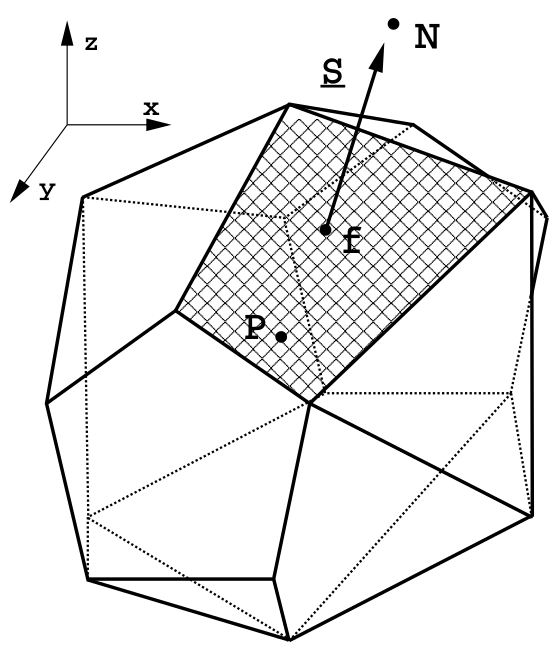
\includegraphics[scale=0.23]{Imagenes/VC_Gral}
                    \end{center}
                \end{figure} 
                                                      
                \column{0.5\textwidth}
                \centering               
                El punto computacional {\bf P} se encuentra en el centroide del volumen de control, tal que
                $$
                \int_{V_p} (\mathbf{x} - \mathbf{x_p})dV = 0
                $$
                No importa la topolog\'ia del VC.
                            
            \end{columns}
        
    \end{itemize}     

\end{frame}















      
\begin{frame}
    \frametitle{M\'etodo de vol\'umenes finitos}
    \framesubtitle{Discretizaci\'on de la ecuaci\'on de transporte}


        \begin{block}{\centering Ecuaci\'on de transporte prototipo}
%        \scriptsize
            $$ \underbrace{\frac{\partial \rho \phi}{\partial t}}_1 + 
               \underbrace{\nabla \cdot (\rho \mathbf{U} \phi)}_2 - 
               \underbrace{\nabla \cdot (\rho \Gamma_{\phi} \nabla \phi)}_3 = 
               \underbrace{S_{\phi}(\phi)}_4$$
        \end{block}          

        \begin{block}{\centering Forma Integral}
            \footnotesize
            $$  \underbrace{ \frac{\partial}{\partial t} \int_{V_{P}}\rho \phi dV}_1 + 
                \underbrace{ \int_{V_{P}}\nabla \cdot (\rho \mathbf{U} \phi) dV }_2 - 
                \underbrace{ \int_{V_{P}}\nabla \cdot (\rho \Gamma_{\phi} \nabla \phi) dV }_3 =  
                \underbrace{ \int_{V_{P}}S_{\phi}(\phi) dV }_4$$
        \end{block} 
    
        
        \begin{enumerate}
            \footnotesize
            \item Derivada temporal
            \item T\'ermino convectivo
            \item T\'ermino difusivo
            \item T\'ermino fuente
        \end{enumerate}      


\end{frame}
    

%---------------------------------------------------------------------------------------------------------------%


\begin{frame}
    \frametitle{M\'etodo de vol\'umenes finitos}
    \framesubtitle{Discretizaci\'on de la ecuaci\'on de transporte}

    Aproximaci\'on de segundo orden

    $$   \phi(\mathbf{x}) = \phi_P + (\mathbf{x} - \mathbf{x}_P) \cdot (\nabla \phi)_P  $$
    $$   \phi (t + \Delta t) = \phi^t + \Delta t (\frac{\partial \phi}{\partial t})^t  $$


    %% con

    %% $$ \phi_P = \phi( \boldsymbol{x_p} ) $$
    %% $$ \phi^t = \phi(t) $$

    Se puede verificar mediante el desarrollo de Taylor de $\phi$

    \begin{align*}
      \phi(\boldsymbol{x}) = \phi_P &+ (\boldsymbol{x} - \boldsymbol{x_p}) \cdot (\nabla \phi)_P + \frac{1}{2}(\boldsymbol{x} - \boldsymbol{x_P})^2 :(\nabla \nabla \phi)_P  \\ 
      & + \frac{1}{3!}(\boldsymbol{x} - \boldsymbol{x_P})^3 ::(\nabla \nabla \nabla \phi)_P \\
      & + ... + \dfrac{1}{n!}(\boldsymbol{x} - \boldsymbol{x_P})^n \underbrace{:::}_n (\underbrace{\nabla \nabla ... \nabla}_n \phi)_P
    \end{align*}
    
    
%    \vspace*{-0.1cm}
%%    \begin{block}{}
%        \footnotesize
%        $$  \underbrace{ \frac{\partial}{\partial t} \int_{V_{P}}\rho \phi dV}_1 + 
%            \underbrace{ \int_{V_{P}}\nabla \cdot (\rho \mathbf{U} \phi) dV }_2 - 
%            \underbrace{ \int_{V_{P}}\nabla \cdot (\rho \Gamma_{\phi} \nabla \phi) dV }_3 =  
%            \underbrace{ \int_{V_{P}}S_{\phi}(\phi) dV }_4$$
%%    \end{block}     
    
    
    %% \begin{columns}

    %%     \column{0.45\textwidth}
    %%         \footnotesize
    %%         \begin{block}{\centering Aproximaci\'on de segundo orden}
    %%              $$   \phi(\mathbf{x}) = \phi_P + (\mathbf{x} - \mathbf{x}_P) \cdot (\nabla \phi)_P $$
    %%              $$   \phi (t + \Delta t) = \phi^t + \Delta t (\frac{\partial \phi}{\partial t})^t $$
    %%         \end{block}                                

    %%     \column{0.45\textwidth}
    %%         \footnotesize
    %%         \begin{block}{}
    %%             \begin{align*}
    %%                  \phi(\mathbf{x}) = & \phi_P + (\mathbf{x} - \mathbf{x}_P) \cdot (\nabla \phi)_P \\
    %%                  &+ \frac{1}{2}(\mathbf{x} - \mathbf{x}_P)^2 :(\nabla \nabla \phi)_P  \\ 
    %%                  &+ \frac{1}{3!}(\mathbf{x} - \mathbf{x}_P)^3 ::(\nabla \nabla \nabla \phi)_P \\
    %%                  &+ ...
    %%             \end{align*}
    %%         \end{block}                                
            
    %% \end{columns}
   
    %% \pause
            
    %% \begin{columns}
    
    %%     \column{0.25\textwidth}
    %%         \begin{figure}[h]
    %%             \begin{center}
    %%                 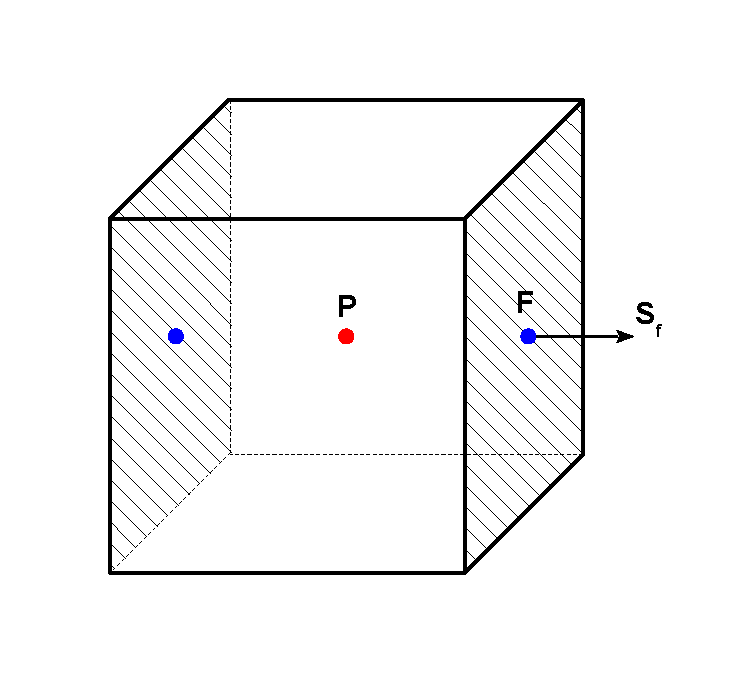
\includegraphics[trim=11mm 11mm 11mm 11mm, clip, scale=0.25]{Imagenes/VF1}
    %%             \end{center}
    %%         \end{figure}         
    
        
    %%     \column{0.7\textwidth}
    %%         \footnotesize
    %%         \begin{block}{Identidades}        
    %%             \begin{align*}
    %%                 \int_{V_P} \phi (\mathbf{x})\,dV &= \int_{V_P} \left [ \phi_P + (\mathbf{x} - \mathbf{x}_P)\cdot (\nabla \phi)_P  \right ] dV = \phi_P V_P
    %%             \end{align*}

    %%             \begin{align*}
    %%                 \int_{V_P} \nabla \cdot \mathbf{a}\,dV &= \sum_f \left( \int_f d\mathbf{S} \cdot \mathbf{a}\right) = \sum_f \mathbf{S} \cdot \mathbf{a}_f
    %%             \end{align*}
                
    %%          \end{block}        
    
    %% \end{columns}
                                                

\end{frame}   







%---------------------------------------------------------------------------------------------------------------%


\begin{frame}
    \frametitle{M\'etodo de vol\'umenes finitos}
    \framesubtitle{Discretizaci\'on de la ecuaci\'on de transporte}

    Discretizaci\'on de los t\'erminos espaciales usando identidades de Gauss

    $$ \int_V \nabla \cdot \boldsymbol{a} dV = \oint_{\partial V} d\boldsymbol{S} \cdot \boldsymbol{a}    \qquad   \int_V \nabla \cdot \phi dV = \oint_{\partial V} d\boldsymbol{S} \phi$$
    $$ \int_V \nabla \boldsymbol{a} dV = \oint_{\partial V} d\boldsymbol{S} \boldsymbol{a}  $$    
    
    \begin{align*}
      \int_{V_P} \phi (\boldsymbol{x})\,dV & = \int_{V_P} \left [ \phi_P + (\boldsymbol{x} - \boldsymbol{x_P})\cdot (\nabla \phi)_P  \right ] dV \\
                                          & = \phi_P \int_{V_P} dV +  \left [  \int_{V_P} (\boldsymbol{x} - \boldsymbol{x_P}) dV \right ] \cdot (\nabla \phi)_P \\
                                          & = \phi_P V_P
    \end{align*}


    %%             \begin{align*}
    %%                 \int_{V_P} \nabla \cdot \mathbf{a}\,dV &= \sum_f \left( \int_f d\mathbf{S} \cdot \mathbf{a}\right) = \sum_f \mathbf{S} \cdot \mathbf{a}_f
    %%             \end{align*}
                
    %%          \end{block}        
    
    %% \end{columns}
                                                

\end{frame}   








%---------------------------------------------------------------------------------------------------------------%


\begin{frame}
    \frametitle{M\'etodo de vol\'umenes finitos}
    \framesubtitle{Discretizaci\'on de la ecuaci\'on de transporte}

    Discretizaci\'on de los t\'erminos espaciales usando identidades de Gauss

    $$ \int_V \nabla \cdot \boldsymbol{a} dV = \oint_{\partial V} d\boldsymbol{S} \cdot \boldsymbol{a}    \qquad   \int_V \nabla \cdot \phi dV = \oint_{\partial V} d\boldsymbol{S} \phi$$
    $$ \int_V \nabla \boldsymbol{a} dV = \oint_{\partial V} d\boldsymbol{S} \boldsymbol{a}  $$    
    
    \begin{align*}
      \int_{V_P} \nabla \cdot \boldsymbol{a}\,dV = \oint_{\partial V} d\boldsymbol{S} \cdot \boldsymbol{a} = \sum_f \left( \int_f d\boldsymbol{S} \cdot \boldsymbol{a} \right)
    \end{align*}

    donde
    \begin{align*}
       \int_f d\boldsymbol{S} \cdot \boldsymbol{a} = \left (  \int_f d\boldsymbol{S} \right ) \cdot \boldsymbol{a_f} + \left [  \int_f d\boldsymbol{S}(\boldsymbol{x} - \boldsymbol{x_f}) \right ] : (\nabla \boldsymbol{a})_f = \boldsymbol{S} \cdot \boldsymbol{a}_f
    \end{align*}
                                                

\end{frame}   










%---------------------------------------------------------------------------------------------------------------%


\begin{frame}
    \frametitle{M\'etodo de vol\'umenes finitos}
    \framesubtitle{Discretizaci\'on del t\'ermino convectivo}
    
    \vspace*{-0.1cm}
    \begin{block}{T\'ermino convectivo}
        \footnotesize
        \begin{equation*}
            \frac{\partial}{\partial t} \int_{V_{P}}\rho \phi dV + 
            \textcolor{red}{ \int_{V_{P}}\nabla \cdot (\rho \bs{U} \phi) dV } - 
            \int_{V_{P}}\nabla \cdot (\rho \Gamma_{\phi} \nabla \phi) dV  =  
            \int_{V_{P}}S_{\phi}(\phi) dV 
        \end{equation*}
    \end{block}     
    

    \footnotesize
    $$ \int_{V_{P}}\nabla \cdot (\rho \bs{U} \phi) dV = \displaystyle \sum_f \bs{S} \cdot (\rho U \phi)_f = \displaystyle \sum_f \bs{S} \cdot (\rho U)_f \phi_f = \sum_f F \phi_f $$

    %% \vspace{0.8cm}
    
    \begin{columns}
            
        \column{0.35\textwidth}
        \vspace*{-0.8cm}
        \begin{figure}[h]
            \begin{center}
                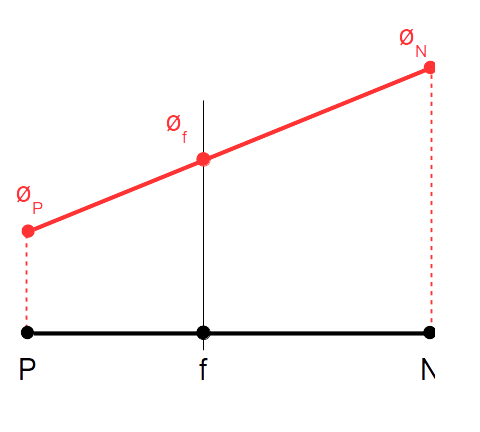
\includegraphics[scale=0.25]{Imagenes/faceflux}
            \end{center}
        \end{figure}     
                                               
        \column{0.6\textwidth}
        \begin{block}{}
          \footnotesize
          \centering Esquemas de interpolaci\'on
          \begin{eqnarray*}
            \phi_f = \frac{\overline{fN}}{\overline{PN}}\phi_P + (1-\frac{\overline{fN}}{\overline{PN}})\phi_N     &     \mbox{\tiny Diferencias centradas}
          \end{eqnarray*}
          \begin{eqnarray*}
            \phi_f = \left \{ 
            \begin{array}{ll} 
              \phi_f = \phi_P & \mbox{si} \, F\geq 0 \\
              \phi_f = \phi_N & \mbox{si} \, F\leq 0 
            \end{array}
            \right .  & \mbox{\tiny Upwind}
          \end{eqnarray*}
        \end{block}

    \end{columns}

\end{frame}       












%---------------------------------------------------------------------------------------------------------------%


\begin{frame}
    \frametitle{M\'etodo de vol\'umenes finitos}
    \framesubtitle{Discretizaci\'on del t\'ermino difusivo}
    
    \vspace*{-0.1cm}
    \begin{block}{T\'ermino difusivo}
        \footnotesize
        \begin{equation*}
            \frac{\partial}{\partial t} \int_{V_{P}}\rho \phi dV + 
            \int_{V_{P}}\nabla \cdot (\rho \bs{U} \phi) dV - 
            \textcolor{red}{ \int_{V_{P}}\nabla \cdot (\rho \Gamma_{\phi} \nabla \phi) dV } =  
            \int_{V_{P}}S_{\phi}(\phi) dV 
        \end{equation*}
    \end{block}     
    

    \footnotesize
    $$ \int_{V_{P}}\nabla \cdot (\rho \Gamma_{\phi} \nabla \phi) dV = \displaystyle \sum_f \bs{S} \cdot (\rho \Gamma_{\phi} \nabla \phi)_f = \displaystyle \sum_f (\rho \Gamma_{\phi})_f \bs{S} \cdot (\nabla \phi)_f $$

    %% \vspace{0.3cm}
    
    \begin{columns}
            
        \column{0.4\textwidth}
        \vspace*{-0.8cm}
        \begin{figure}[h]
            \begin{center}
                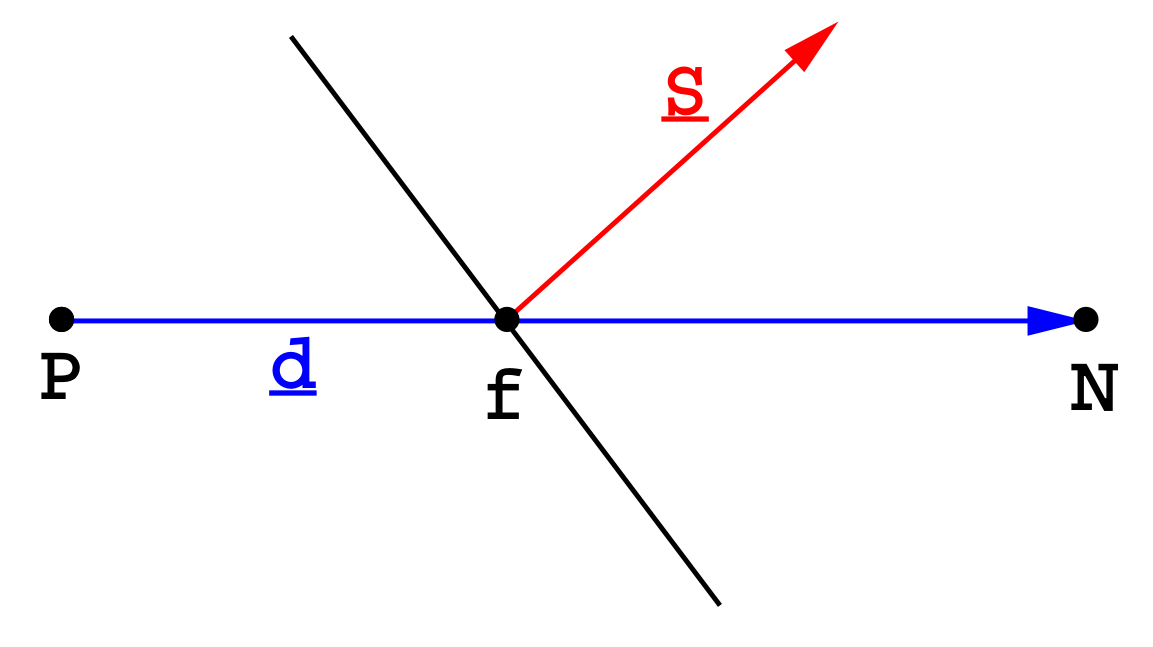
\includegraphics[width=0.98\textwidth]{Imagenes/face_S_d}
            \end{center}
        \end{figure}     
                                               
        \column{0.5\textwidth}
        \begin{block}{}
          \footnotesize
          \centering Si la malla es ortogonal ($\bs{d} \parallel \bs{S}$)
          $$  \bs{S} \cdot (\nabla \phi)_f = \frac{|\bs{S}|}{|\bs{d}|} (\phi_N - \phi_P)  $$
          o bien
          $$  (\nabla \phi)_P = \frac{1}{V_P} \sum_f \bs{S} \phi_f  $$
          $$  (\nabla \phi)_f = f_x (\nabla \phi)_P + (1-f_x)(\nabla \phi)_N  $$
        \end{block}
    \end{columns}

\end{frame}       





%---------------------------------------------------------------------------------------------------------------%


\begin{frame}
    \frametitle{M\'etodo de vol\'umenes finitos}
    \framesubtitle{Discretizaci\'on del t\'ermino difusivo}

    \begin{center}
      \textcolor{red}{Desafortunadamente, una malla ortogonal es m\'as excepci\'on que regla}
    \end{center}
    
    Se divide el operador en dos partes
    $$ \bs{S}_f \cdot (\nabla \phi)_f = \underbrace{\bs{\Delta} \cdot (\nabla \phi)_f}_{\mbox{\tiny Contribuci\'on ortogonal}} + \underbrace{\bs{k} \cdot (\nabla \phi)_f}_{\mbox{\tiny Contribuci\'on no ortogonal}} $$

    $$ \bs{S} = \bs{\Delta} + \bs{k} $$

    Con esta aproximaci\'on se elije $\bs{S} \parallel \bs{\Delta}$ de forma de usar la representaci\'on ortogonal en el primer t\'ermino. Se plantean 3 formas para representar la contribuci\'on no ortogonal

\end{frame}






%---------------------------------------------------------------------------------------------------------------%


\begin{frame}
    \frametitle{M\'etodo de vol\'umenes finitos}
    \framesubtitle{Discretizaci\'on del t\'ermino difusivo}

    \textbf{Correcci\'on m\'inima}
    
    \begin{columns}

    \column{0.45\textwidth}
    \begin{figure}[h]
      \begin{center}
        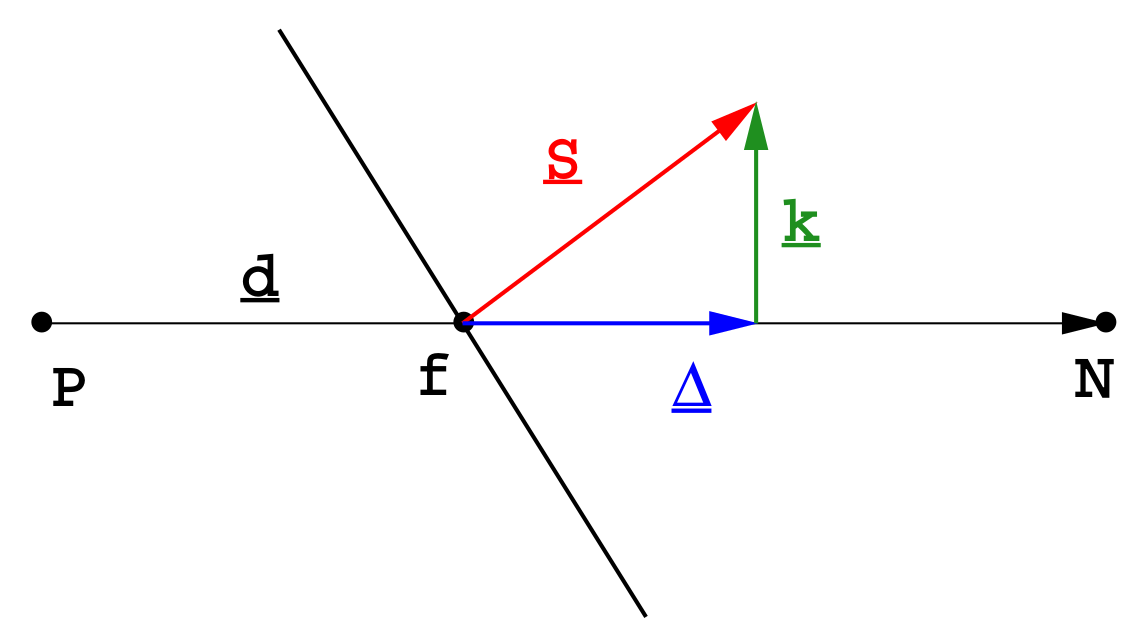
\includegraphics[width=0.95\textwidth]{Imagenes/CorreccionMinima}
      \end{center}
    \end{figure}


    \column{0.45\textwidth}
    \begin{center}
      Minimiza la contribuci\'on no ortogonal usando $\bs{\Delta} \perp \bs{k}$
    \end{center}

    $$ \bs{\Delta} = \dfrac{ \bs{d} \cdot \bs{S}_f }{\bs{d} \cdot \bs{d}} \bs{d} $$

    \end{columns}
    



    \textbf{Correcci\'on ortogonal}
    
    \begin{columns}

    \column{0.45\textwidth}
    \begin{figure}[h]
      \begin{center}
        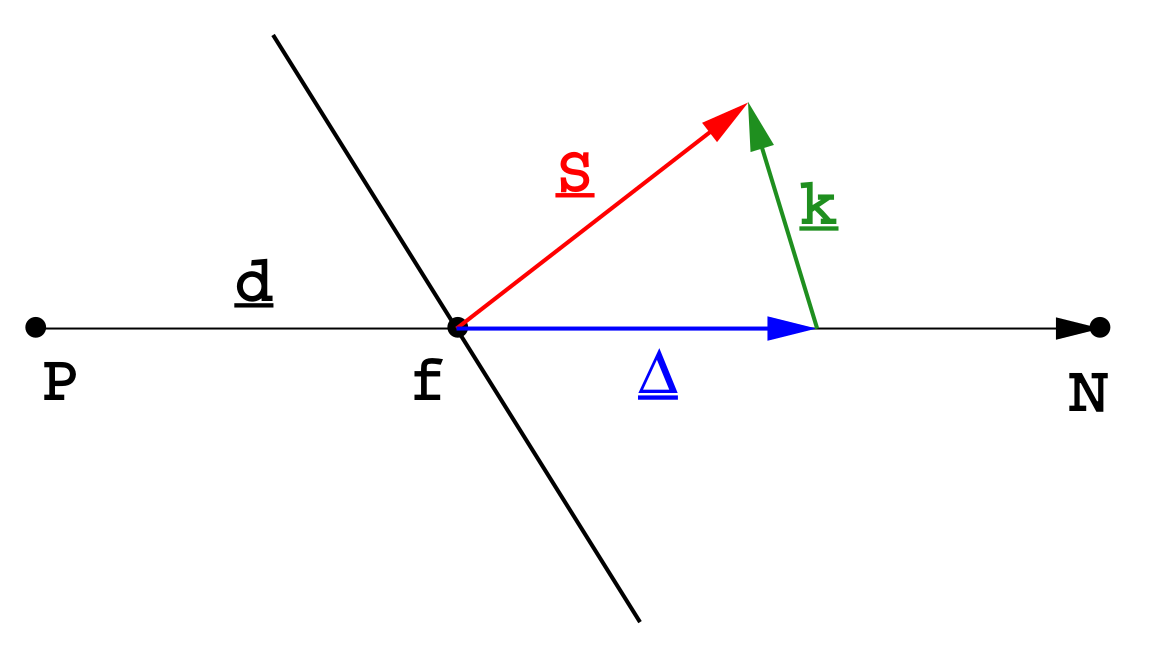
\includegraphics[width=0.95\textwidth]{Imagenes/CorreccionOrtogonal}
      \end{center}
    \end{figure}


    \column{0.45\textwidth}
    \begin{center}
      Conserva la contribuci\'on de $\phi_P$ y $\phi_N$ respecto a la contribuci\'on ortogonal
    \end{center}

    $$ \bs{\Delta} = \dfrac{ \bs{d} }{ |\bs{d}| } |\bs{S}| $$

    \end{columns}
    
\end{frame}










%---------------------------------------------------------------------------------------------------------------%


\begin{frame}
    \frametitle{M\'etodo de vol\'umenes finitos}
    \framesubtitle{Discretizaci\'on del t\'ermino difusivo}

    
    \textbf{Correcci\'on sobre-relajada}
    
    \begin{columns}

    \column{0.45\textwidth}
    \begin{figure}[h]
      \begin{center}
        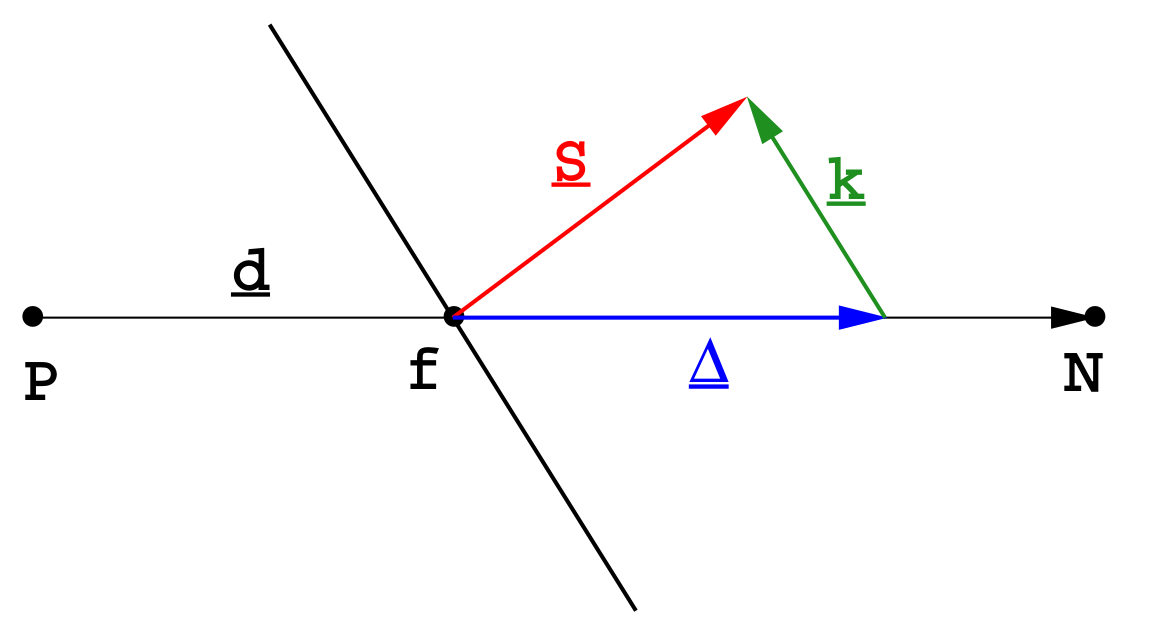
\includegraphics[width=0.95\textwidth]{Imagenes/CorreccionSobreRelajada}
      \end{center}
    \end{figure}


    \column{0.45\textwidth}
    \begin{center}
      La contribuci\'on de $\phi_P$ y $\phi_N$ crece con la no ortogonalidad
    \end{center}

    $$ \bs{\Delta} = \dfrac{ \bs{d} }{\bs{d} \cdot \bs{S}} |\bs{S}|^2 $$

    \end{columns}
    

    En definitiva
    $$ \bs{S} \cdot (\nabla \phi)_f = |\bs{\Delta}| \dfrac{ \phi_N - \phi_P }{ |\bs{d}| }  +  \bs{k} \cdot (\nabla \phi)_f$$

    con
    $$  (\nabla \phi)_f = f_x (\nabla \phi)_P + (1-f_x)(\nabla \phi)_N  \qquad   (\nabla \phi)_P = \frac{1}{V_P} \sum_f \bs{S} \phi_f  $$    


    
\end{frame}











%---------------------------------------------------------------------------------------------------------------%


\begin{frame}
    \frametitle{M\'etodo de vol\'umenes finitos}
    \framesubtitle{Discretizaci\'on del t\'ermino fuente}
    
    \vspace*{-0.1cm}
    \begin{block}{}
        \footnotesize
        \begin{equation*}
           \frac{\partial}{\partial t} \int_{V_{P}}\rho \phi dV + 
             \int_{V_{P}}\nabla \cdot (\rho \mathbf{U} \phi) dV  - 
             \int_{V_{P}}\nabla \cdot (\rho \Gamma_{\phi} \nabla \phi) dV =  
             \textcolor{red}{ \int_{V_{P}}S_{\phi}(\phi) dV}
        \end{equation*}
    \end{block}     
    
    
    \begin{columns}
            
        \column{0.35\textwidth}
        \begin{figure}[h]
            \begin{center}
                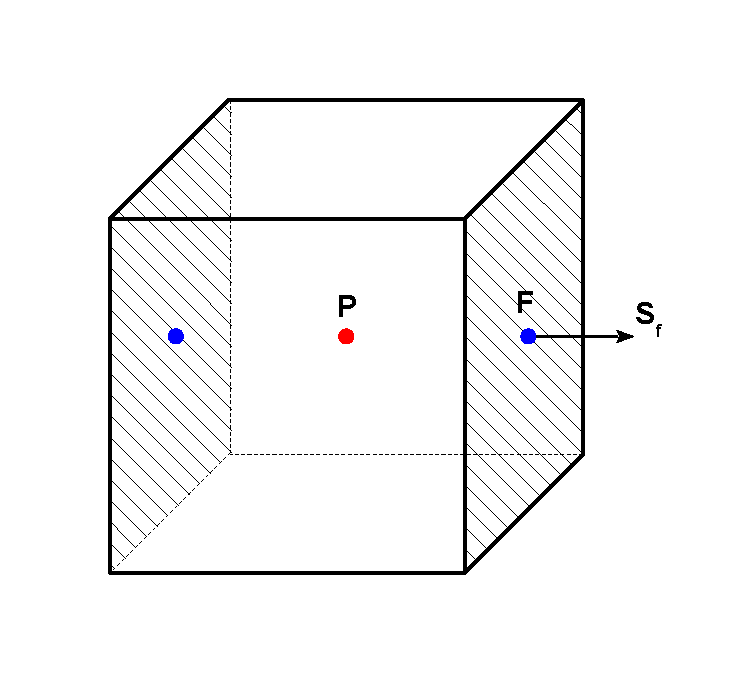
\includegraphics[trim=11mm 11mm 11mm 11mm, clip, scale=0.25]{Imagenes/VF1}
            \end{center}
        \end{figure} 
        \vspace*{-0.8cm}
        \begin{figure}[h]
            \begin{center}
                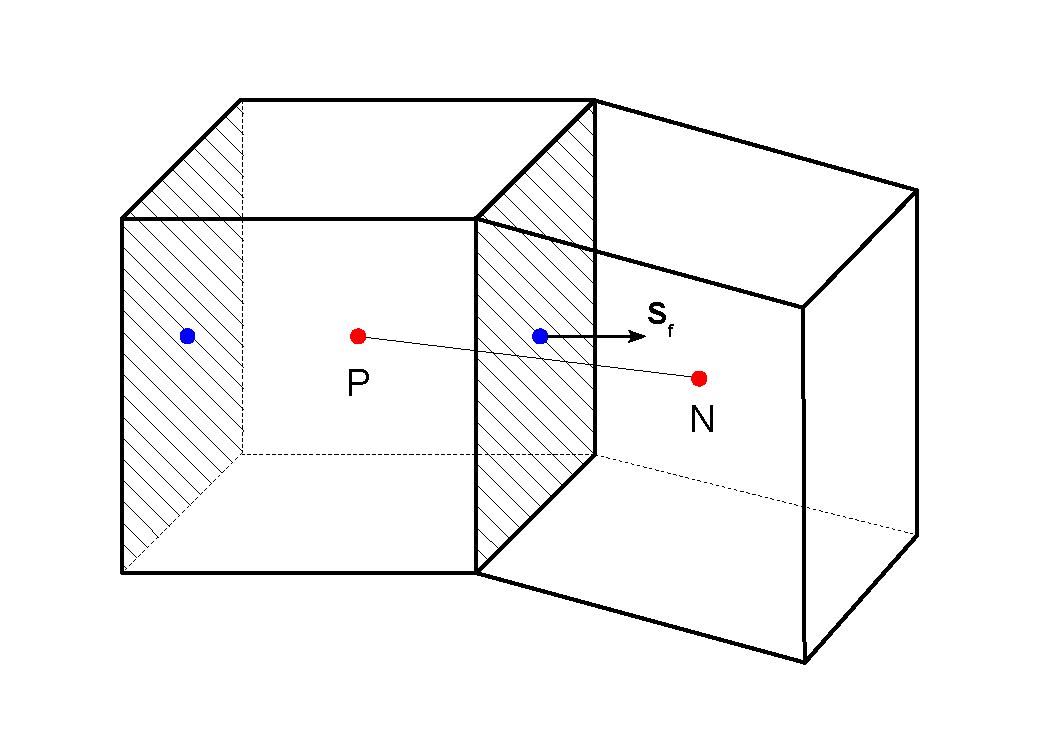
\includegraphics[trim=10mm 10mm 10mm 10mm, clip, scale=0.25]{Imagenes/VF2}
            \end{center}
        \end{figure}         
                                               
        \column{0.6\textwidth}
            \footnotesize
            \begin{block}{\centering T\'ermino fuente}
                \begin{equation*}
                    S_{\phi}(\phi) = Su + Sp\phi
                \end{equation*}
                \begin{equation*}
                     \int_{V_{P}}S_{\phi}(\phi) dV = Su\, V_P + Sp\, V_P\phi_P
                \end{equation*}
            \end{block}                                

            Se realiza una linealizaci\'on del t\'ermino fuente, previa a la discretizaci\'on.
    \end{columns}

\end{frame}       




%---------------------------------------------------------------------------------------------------------------%


\begin{frame}
    \frametitle{M\'etodo de vol\'umenes finitos}
    \framesubtitle{Discretizaci\'on temporal}
       
    \begin{exampleblock}{\centering Semi-discretizaci\'on temporal}
        \tiny
        \begin{equation*}
            \int_t^{t+\Delta t}\left [ \left ( \frac{\partial \rho \phi}{\partial t} \right)_P V_{P} + 
            \displaystyle \sum_f \mathbf{S}_f \cdot (\rho U)_f \phi_f - 
            \displaystyle \sum_f (\rho \Gamma_{\phi})_f \, \mathbf{S}_f \cdot (\nabla \phi)_f \right]  dt= 
            \int_t^{t+\Delta t}\left ( Su\, V_P + Sp\, V_P\phi_P \right ) dt 
        \end{equation*}
    \end{exampleblock}        

    \begin{block}{Crank-Nicolson}
        \footnotesize
        \begin{eqnarray*}
            \frac{\rho_P \phi_P^n - \rho_P \phi_P^0}{\Delta t}V_P 
            + 
            \frac{1}{2} \displaystyle \sum_f \mathbf{S}_f \cdot (\rho U)_f \phi_f^n 
            - 
            \frac{1}{2} \displaystyle \sum_f (\rho \Gamma_{\phi})_f \, \mathbf{S}_f \cdot (\nabla \phi)_f^n 
            +
            \frac{1}{2} \displaystyle \sum_f \mathbf{S}_f \cdot (\rho U)_f \phi_f^0             \\
            - 
            \frac{1}{2} \displaystyle \sum_f (\rho \Gamma_{\phi})_f \, \mathbf{S}_f \cdot (\nabla \phi)_f^0  
            =
            Su\,V_P 
            +
            \frac{1}{2}Sp\, V_P\phi_P^n
            +
            \frac{1}{2}Sp\, V_P\phi_P^0
        \end{eqnarray*}
    \end{block}  
    
    $$
    a_P \phi_P^n + \sum_N a_N \phi_N^n = R_P  \rightarrow [A][\phi] = [R]
    $$  

\end{frame}




\input CondicionDeBorde

\input ErroresMalla

\input NavierStokes
